%--------------------------------------
% Create title frame
\titleframe

%--------------------------------------
% Table of contents
\begin{frame}{Overview}
  \setbeamertemplate{section in toc}[sections numbered]
  \tableofcontents[hideallsubsections]
\end{frame}



%--------------------------------------


\begin{frame}{This lecture expands on}
    \begin{itemize}
      \item Lecture notes of Pr. Thierry Van Cutsem
      \item Chapter 12 from the Ned Mohan's book (summarized by Pr. Louis Wehenkel).
      \item Mohan, Ned. Electric power systems: a first course. John Wiley \& Sons, 2012.
    \end{itemize}
\end{frame}


\section{Why do we need to control power systems?}

% Why and how to control voltage and frequency?
\begin{frame}{Why to control power systems?}
  \begin{itemize}
      \item Technical requirements: power system devices are designed so as to operate within well-defined "tolerance regions" 
      \begin{itemize}
        \item around nominal values of voltage $V_n$: $1 \pm 0.1$ pu in Europe
        \item around nominal value of frequency $f_n$: $50 \pm 0.2$  Hz in Europe (in steady state)
        \item within the $P$-$Q$ capabilities of devices
        \item under the current limits of lines and transformers
      \end{itemize} 
      \item Large/persistent deviations from nominal values could lead to 
      \begin{itemize}
        \item damages and safety problems (e.g. high voltage)
        \item cascading phenomena
        \item service interruptions
      \end{itemize}
      
  \end{itemize}
\end{frame}

\begin{frame}{Exogeneous threats}
  \begin{itemize}
      \item Sudden disturbances, such as line or generator tripping
      \item Fast variations of the \textit{net load} (cf. Duck curve)
      \begin{itemize}
        \item the net load refers to the load "seen" by the transmission system, i.e. the load minus the non-controllable dispersed generation
      \end{itemize}
      \item weather conditions, such as storms, which can impact the generation of renewable energy sources (RES) (e.g. wind turbines' cut-out speed)
  \end{itemize}
\end{frame}

% Impact of the storm on wind generation
\begin{frame}{Impact of a storm on wind generation}
  \begin{columns}
  \begin{column}{0.5\textwidth}
      \begin{itemize}
        \item On November 2, 2023, a storm hit Belgium, causing a significant drop in wind generation.
        \item Wind generation dropped from 4.5 GW to 0.5 GW in less than 30 minutes.
        \item This sudden drop required immediate action to maintain the power balance and frequency stability.
    \end{itemize}
    
  \end{column}
  \begin{column}{0.5\textwidth}
    \begin{center}
        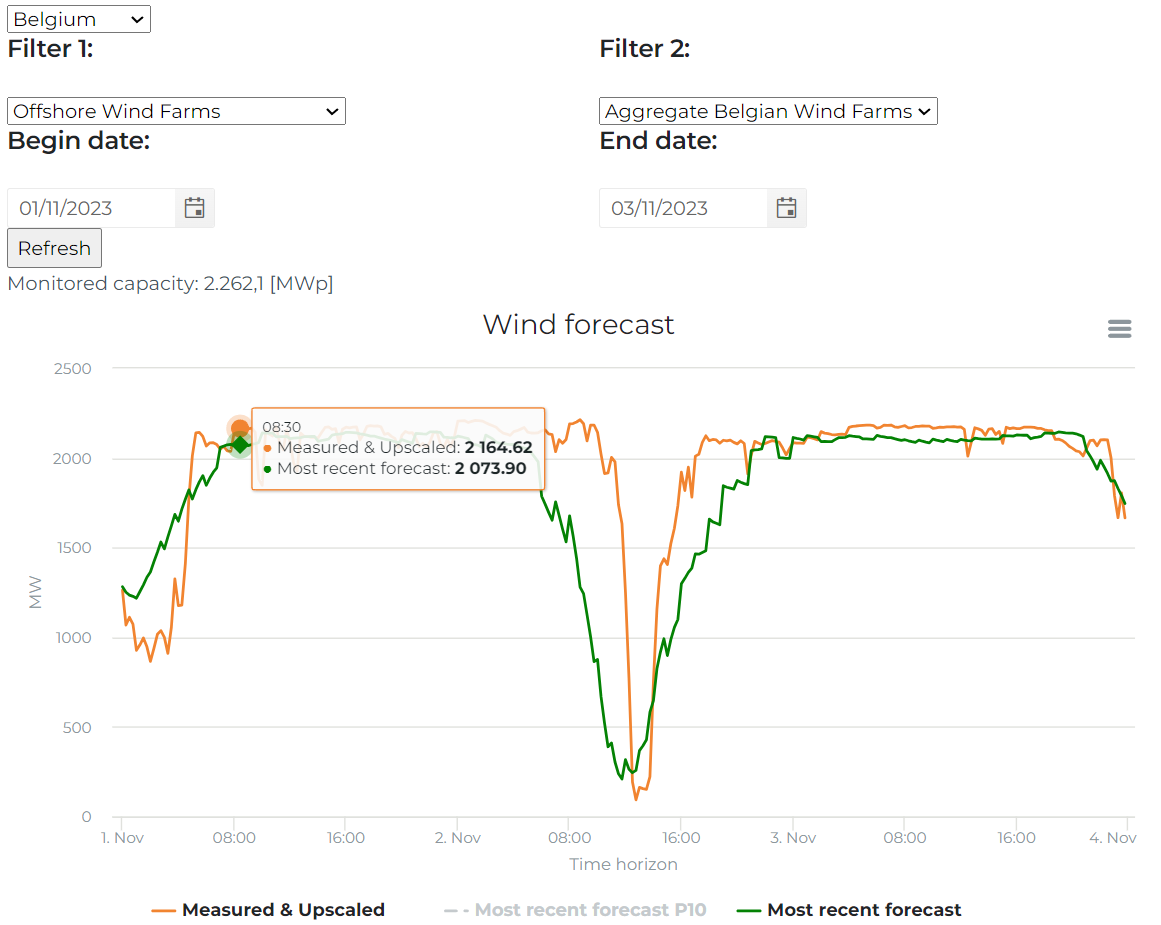
\includegraphics[width=\textwidth]{images/elia_storm_offshorewind_20231102.PNG}
    \end{center}
  \end{column}
\end{columns}
{\small From \url{https://www.elia.be/en/grid-data/power-generation/wind-power-generation}}
    
\end{frame}


\begin{frame}{Control resources}

    Several control resources are available to maintain the system within acceptable limits, and to restore them to nominal values after a disturbance.
      \begin{itemize}
          \item Adjust synchronous generators' field current
          \item Adjust synchronous generators' mechanical power
          \item Change transformer taps
          \item Change shunt compensation
          \item Act on topology: switch lines and transformers in/out of service
          \item Fast start-up generator units 
          \item In extremis load curtailment
          \item Control renewable generation (e.g. PV curtailment)
          \item Use batteries and other energy storage systems %TODO Ask ELIA to which reserve markets batteries are participating
      \end{itemize}
\end{frame}

\begin{frame}{How to use these control resources?}
    \begin{itemize}
      \item But which control resources to use, and when? 
      \item What will have an effect on frequency and voltage? 
      \item How to coordinate them?
    \end{itemize}

    \begin{block}{Focus of the lecture}
      In this lecture we will focus on the frequency control, and we will see how it is related to the power balance in the system.
    \end{block}
    Later, we will adress voltage control and also introduce other problems related to transient stability.
\end{frame}

\section{The link between frequency and power balance}

\begin{frame}
  \frametitle{Frequency and power}
  
    The frequency of the grid is tightly linked to the \textbf{active} power balance in the system.
  
    \begin{itemize}
        \item Electrical energy cannot be stored (in large quantities)
        \item it is produced when it is requested 
        \item in the very first instants after a disturbance, the missing (resp. excess) energy is taken from (resp. stored into) the rotating masses of the synchronous machines 
        \item this causes a variation of their speed of rotation, and hence of frequency 
        \item this is sensed by the speed governors (en français: régulateurs de vitesse), which adjust the steam/water/gas flow in the turbines to correct the speed deviation
        \item Other mechanisms are used to restore the power balance and the frequency to nominal values
    \end{itemize}
    

\end{frame}

\begin{frame}
  \frametitle{Frequency correction is performed in three steps}

  Three reserve mechanisms are used to correct the frequency deviation and restore the power balance:

  \begin{itemize}
      \item primary reserve (in a few seconds): local/decentralized, speed control in power plants 
      \item secondary reserve (in a few minutes): distributed: corrections of generator power setpoints to restore frequency and power exchanges to nominal values
      \item tertiary reserve (in a few tens of minutes): centralized: re-optimization of generation and exchange schedules, while restoring secondary control reserves
  \end{itemize}

  \begin{center}

    \begin{tabular}{|l|l|}
      \hline
      \textbf{Reserve Level} & \textbf{Current Name (ENTSO-E)} \\
      \hline
      Primary Reserve   & Frequency Containment Reserve (FCR) \\
      Secondary Reserve & Automatic Frequency Restoration Reserve (aFRR) \\
      Tertiary Reserve  & Manual Frequency Restoration Reserve (mFRR) \\
      \hline
    \end{tabular}
  \end{center}

\end{frame}
      
      

% System frequency evolution: theory, example, and intuition
\begin{frame}
    \frametitle{System frequency evolution: theory, example, and intuition}
    Before understanding in more details these three levels, we will try to get intuition based on a simplified physical model of the system.
    
    Let us consider a power system with loads and, for now, only synchronous generators.

    Let
    \begin{itemize}
        \item $p_e(t)$ be the total power absorbed by the loads (incl. losses in the network and conversion losses in the generators)
        \begin{itemize}
            \item this is thus equal to the electrical power that generators must output (Kirchhoff laws)
        \end{itemize}
        \item $p_m(t)$ be the mechanical power input to generators
    \end{itemize}
    Except for the losses mentioned above, we neglect the network.

    \textbf{How does the frequency of the system $f(t)$ (and thus of the machines) evolve?}
\end{frame}


% The swing equation
\begin{frame}[allowframebreaks]{The swing equation}

    We consider a synchronous power system that should operate at the nominal frequency $f_N$.
    To simplify, we will group all synchronous generators into a single equivalent generator with an
    inertia constant $J$. %()

    Newton's law $$J\alpha = T_m-T_e,$$ 
    relates the angular acceleration $\alpha$ of the rotor to the difference between the mechanical torque $T_m$ and the electrical torque $T_e$.
    
    Since $p = T\omega$ and $\omega = 2\pi f$, we can derive a more convenient expression linking the frequency and the active power balance in the system:
    $$J \frac{df}{dt} = \frac{p_m - p_e}{4\pi^2 f}$$

    We must correct this expression to include the damping effect in generators, assuming $D_g$ is an equivalent total damping coefficient of the system: 
    $$J \frac{df}{dt} = \frac{p_m - p_e}{4\pi^2 f} \color{red}{- D_g (f-f_N)}$$

\end{frame}
\begin{frame}{What happens if ...}

    \begin{block}{What happens in case there is a power imbalance?}
    E.g. a sudden increase of load? \vspace*{1cm}
    \end{block}
    
    \begin{block}{What is the effect of inertia?}
      \vspace*{1cm}
    \end{block}

    \begin{block}{What is the effect of samping?}
      \vspace*{1cm}
    \end{block}

\end{frame}

\begin{frame}{Note: Inertia constant of a generator}

  The inertia constant \( J_i \) of generator \( i \) can be expressed as a function of its rated power \( P_{\max,i} \) and its dimensionless inertia constant \( H_i \). The relationship is given by:
\[
J_i = \frac{2 P_{\max,i} H_i}{4 \pi^2 f_N^2}
\]
where \( f_N \) is the nominal grid frequency, typically 50 or 60 Hz. 
This formula converts the per-unit inertia constant \( H_i \), which represents the stored kinetic energy at rated power in seconds, into the physical moment of inertia \( J_i \) in SI units (kg m$^2$) , assuming a synchronous speed of \( 2\pi f_N \) radians per second.

In the Swing equation, we have considered that $J = \sum_i J_i$.

\end{frame}

% To answer these questions, let's look at some simulations
\begin{frame}
    \frametitle{To answer these questions, let's look at some simulations}
    \href{https://colab.research.google.com/drive/1vARBr5wfm9uHCokRx3kcoK_RWjrOvnA5}{\color{blue}{Link to the simulations}}

    The code is organized in 3 main parts:
    \begin{enumerate}
        \item Plotting functions
        \item A class encoding the power system data and the set of differential equations governing the system
        \item Simulations for several cases
    \end{enumerate}
\end{frame}

\begin{frame}{Let's add generator reaction to frequency change}

  \begin{itemize}
    \item So far, only the generator's inertia and damping were considered.
    \item This is not enough to stabilize the frequency.
    \item Hence, generators react to frequency changes by adjusting their mechanical power output.
    \item The first reaction is the primary control. Let's understand how a power plant is modeled and controlled.
  \end{itemize}
\end{frame}

\begin{frame}
    \frametitle{Speed governor of a synchronous generator}
    \begin{columns}
        \begin{column}{0.55\textwidth}
            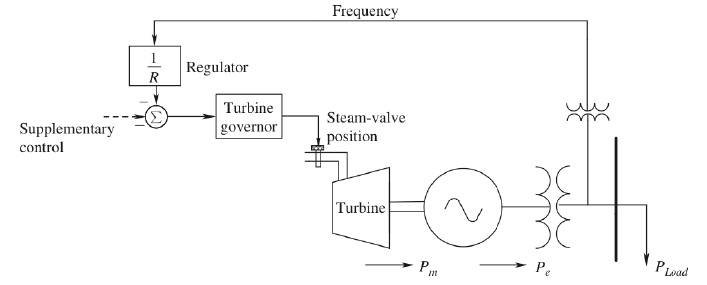
\includegraphics[width=\textwidth]{images/governor.png}
        \end{column}
        \begin{column}{0.4\textwidth}
            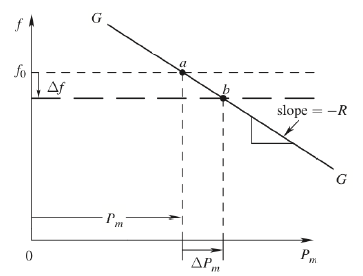
\includegraphics[width=\textwidth]{images/droop-1gen.png}
        \end{column}
    \end{columns}
    \begin{itemize}
        \item Measurement of rotor speed (or stator frequency as a proxy)
        \item If frequency (speed) is a bit below $f_0$, the governor opens a bit more the valve to increase the mechanical power $P_m$
        \item In steady state, speed and mechanical power (or equivalently, frequency and electric power) are related by a linear relationship (see diagram on the right)
        \item This relationship allows predicting how the power generated by a certain generator would change when frequency changes
        \item It also shows that in order to have the generator adapt his power via this primary control loop, the frequency must change
    \end{itemize}
\end{frame}

\begin{frame}{Model of a power plant (mechanical part)}
  \begin{columns}
    \begin{column}{0.48\textwidth}
      The mechanical part of a power plant is modeled by the following block diagram:
      \begin{center}
        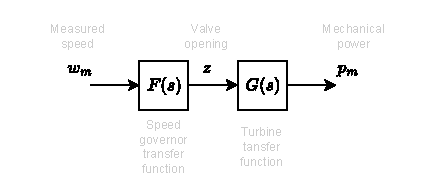
\includegraphics[width=0.85\textwidth]{images/governor_and_turbine_transfer_function.pdf}    
      \end{center}
    \end{column}
    \begin{column}{0.48\textwidth}
      \begin{itemize}
        \item $\omega_{m}$ is the rotation speed (which is not necessarily equal to the grid angular speed $\omega$ (in rad/s) depending on the number of poles of the alternator)
        \item $z$ is the fraction of opening of the turbine control valves ($0\le z\le1$), to inject e.g. more steam in the turbine.
      \end{itemize}
      We will not delve deeper into the turbine model, but focus on the speed governor.
    \end{column}
  \end{columns}
\end{frame}

\begin{frame}{Speed governor transfer function}
    \begin{columns}
    \begin{column}{0.6\textwidth}
    \begin{center}
      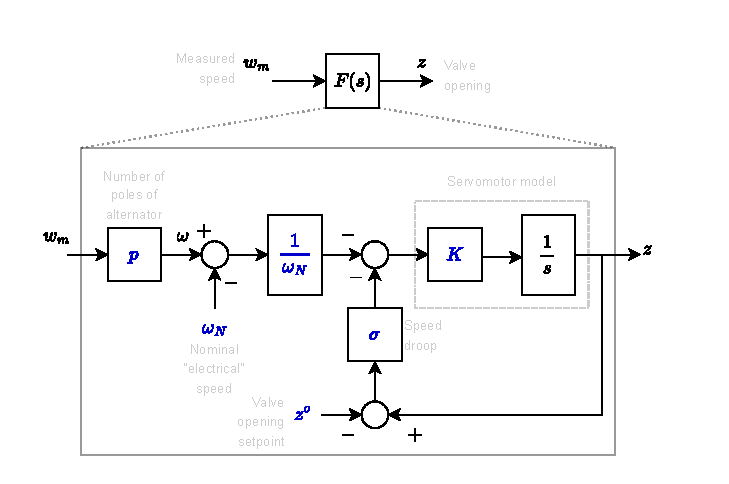
\includegraphics[width=\textwidth]{images/speed_governor_transfer_function.pdf}    
    \end{center}
    \end{column}
    \begin{column}{0.35\textwidth}
      \color{blue}{Parameters are in blue.}
    \end{column}
    \end{columns}
\end{frame}

\begin{frame}{Speed governor transfer function (...)}
    \begin{itemize}
      \item The rotation speed is scaled and compared to the nominal electrical speed to yield a speed error signal
      \item $z^o$ sets the desired power production setpoint of the generator, if the frequency were at nominal value
      \item In the feedback branch, $z$ is compared to $z^o$ and scaled by the droop coefficient $\sigma$ to yeald a second error signal
      \item The error signals are then fed to the servomotor to adjust $z$        
    \end{itemize}
\end{frame}


\begin{frame}{Equivalent block diagram}
  We can redraw the diagram in an equivalent manner, with $T_{sm} = 1/(K \sigma)$ the time constant of the servomotor, as 
  \begin{center}
        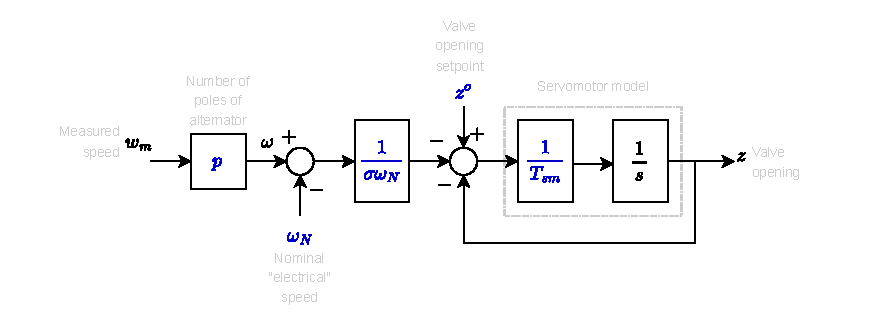
\includegraphics[width=0.9\textwidth]{images/speed_governor_transfer_function_2.pdf}    
  \end{center}
\end{frame}

\begin{frame}{Equivalent block diagram (...)}
  The transfer function of the speed governor is then:
  $$z = F(s) = \frac{1}{1 + s T_{sm}} \left( z^{o} - \frac{\omega - \omega_{N}}{\sigma \omega_{N}} \right)$$
  
  \begin{block}{Exercise}
  Obtain this transfer function from the previous diagram, and show it is equivalent to the first diagram.
  \end{block}
\end{frame}

\begin{frame}{Steady-state characteristic of a turbine-governor set}
      \begin{columns}
    \begin{column}{0.65\textwidth}


    In steady state:
    \begin{itemize}
      \item $p_m = G(0)z$ (remember $G(s)$ models the turbine) 
      \item $z = F(0) = z^o - \frac{\omega - \omega_N}{\sigma \omega_N}$ 
    \end{itemize}
    For $z = 1$, $p_m = P_N$, the nominal power of turbine (MW) \\ 
    Hence, $P_N = G(0) 1$  and $$p_m = P_N z$$ 
    
    Thus, $p_m = P_N z^o - \frac{P_N}{\sigma} \frac{\omega - \omega_N}{\omega_N}$
    or $$p_m = P_o - \frac{P_N}{\sigma} \frac{f - f_N}{f_N}$$
    where $P_o$ is the power setpoint of the generator.
    
    \end{column}
    \begin{column}{0.33\textwidth}

        Of course, we must account for the limits of the generator.
        \begin{center}  
          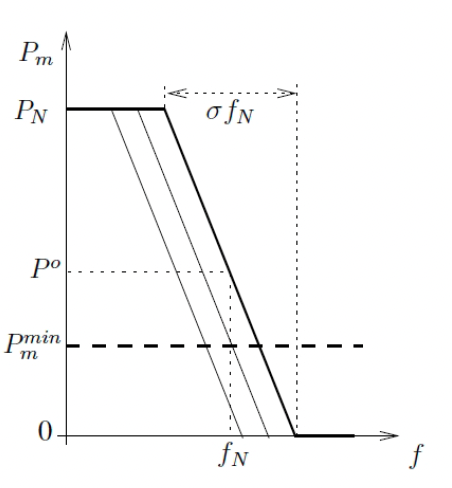
\includegraphics[width=\textwidth]{images/generator_droop_steady_state.png} % Replace with your image file
        \end{center}
          
    \end{column}
    \end{columns}
\end{frame}


% Let's add generator reaction to frequency change
\begin{frame}{Time domain turbine-governor model}

    Back to the time domain, we can write the following differential equation for the mechanical power output of the generator:
    $$T_{sm} \frac{d p_m}{dt} = P^0 - p_m - \frac{P_{N}}{\sigma}\frac{f-f_N}{f_N}$$
    Typical values are: $T_{sm} \approx 1.5 $ s, $\sigma \approx 4\%$.

    \begin{block}{What is the impact of primary control and of the value of $\sigma$?}
      \vspace*{1cm}
    \end{block}

    
\end{frame}

% We should not forget generator limits
\begin{frame}
    \frametitle{We should not forget generator limits}
    $$p_m \in [P_{\min}, P_{\max}]$$
    Where
    \begin{itemize}
        \item $P_{\max}$ the maximum power available for primary control
        \item $P_{\min}$ the minimum power available for primary control
    \end{itemize}

    \begin{block}{What is the consequence of these limits?}
      \vspace*{1cm}
    \end{block}

\end{frame}

 \begin{frame}[allowframebreaks]{About the speed droop $\sigma$ (en français: le statisme)}
    
    \begin{block}{Speed droop $\sigma$}
        The speed droop is the ratio between the relative frequency deviation and the relative power deviation.
        $$\sigma = \left| \frac{\Delta f / f_N}{\Delta P_m/P_N} \right| = \left| \frac{\Delta \omega/\omega_N}{\Delta P_m/P_N} \right|$$
        \begin{itemize}
            \item $\Delta f$ is the frequency deviation from nominal value $f_N$.
            \item $\Delta P_m$ is the mechanical power deviation from nominal value $P_N$.
        \end{itemize}
    \end{block}
  
  \begin{itemize}
    \item A frequency deviation $\Delta f = \sigma f_N = 0.04 \times 50 = 2$ Hz would result in a variation of mechanical power $\Delta P_m = P_N$.
    \item if $\sigma \rightarrow \infty$ the machine operates at constant power, and does not participate in frequency control.
  \end{itemize}    
    
    \begin{block}{The speed controller is of the proportional type}
    \begin{itemize}
        \item it leaves a steady-state frequency error, but . . . 
        \item this is precisely the signal allowing to share the effort over the various generators.
    \end{itemize}
  \end{block}
\end{frame}

% But the power consumed by the load is frequency dependent
\begin{frame}
    \frametitle{The power consumed by the load is frequency dependent}
    $$p_e = P_e^0 (1+D_l (f-f_N) )$$
    where:
    \begin{itemize}
        \item $P^0_{e}$ nominal (or initial) consumption
        \item $D_l$ the sensitivity of consumption to frequency, assumed equal to $1\%$.
    \end{itemize}
    Not all loads are frequency dependent.

    \begin{block}{Do you see the impact on the curves? }
    \vspace*{1cm}
    \end{block}
    
\end{frame}

% Let's now add renewable generation
\begin{frame}{The impact of renewable generation}
    Assume we now have $p_{PV}(t)$ generated by a PV farm.

    \textbf{Which equation does it impact?}

    Our model so far:
    \begin{align*}
    J \frac{df}{dt} &= \frac{p_m - p_e}{4\pi^2 f} - D_g (f-f_N)\\
    T_{sm} \frac{d p_m}{dt} &= P^0_m - p_m - \frac{P_{N}}{\sigma}\frac{f-f_N}{f_N}\\
    p_m &\in [P_{\min}, P_{\max}]\\
    p_e &= P_e^0 (1+D_l (f-f_N) )
    \end{align*}
\end{frame}

% Let's now add renewable generation (continued)
\begin{frame}
    \frametitle{Let's now add renewable generation}
    Assume we now have $p_{PV}(t)$ generated by a PV farm.

    \textbf{Which equation does it impact? }
    $$J \frac{df}{dt} = \frac{p_m - p_e \color{red}{+ p_{PV}}}{4\pi^2 f} - D_g (f-f_N)$$
    \begin{block}{What is the consequence?}
    \vspace*{1cm}
    \end{block}
\end{frame}

% Let's add over frequency curtailment of renewable generation
\begin{frame}{Renewables also have to participate to frequency control}
  \begin{columns}
  \begin{column}{0.55\textwidth}
    \begin{center}
      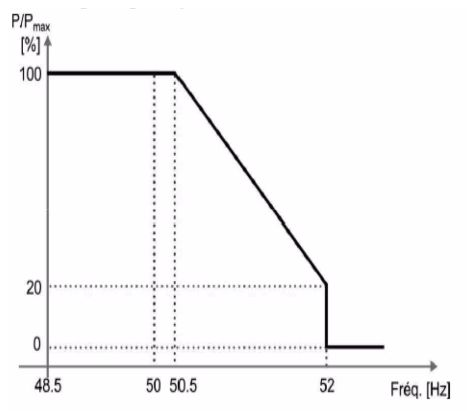
\includegraphics[width=0.8\textwidth]{images/diagramPf.PNG}
    \end{center}
    \end{column}
    \begin{column}{0.4\textwidth}
      \textbf{Over frequency curtailment of renewable generation}
      \end{column}
  \end{columns}
\end{frame}

% Let's add over frequency curtailment of renewable generation: model
\begin{frame}
    \frametitle{Let's add over frequency curtailment of renewable generation: model}
    if $f < 50.5 Hz$:
    $$p_{PV} = P^0_{PV} $$
    else if $ 50.5 \leq f < 52 Hz$:
    $$p_{PV} = P^0_{PV} \left(1 - \frac{0.8}{1.5}(f-50.5)\right) $$
    else if $f \geq 52 Hz$:
    $$p_{PV} = 0.0$$
    where $P^0_{PV}$ is the maximum possible solar output (MPPT) at the initial instant of simulation.

    Note: With more RES, less synchronous machine, so relatively less inertia for same demand.
\end{frame}


\section{Primary frequency control}

\begin{frame}{Objective and assumptions}

    This section aims at understanding the properties of primary frequency control, which has been introduced in the previous section.

    Assumptions: 
    \begin{itemize}
      \item the system has come back to steady state 
      \item we consider several machines, and they all have the same electrical speed
      \item all machines participate in primary frequency control
      \item the network is lossless 
      \item the mechanical power produced by the turbines is completely converted into electrical power 
      \item load is sensitive to frequency as introduced in the previous section
      \item the system initially operates at the nominal frequency ($f = f_N$), for simplicity
    \end{itemize}
\end{frame}


% The case of two generators helping out with a sudden increase of load
\begin{frame}[allowframebreaks]{The case of two generators helping out with a sudden increase of load}
    \begin{center}
        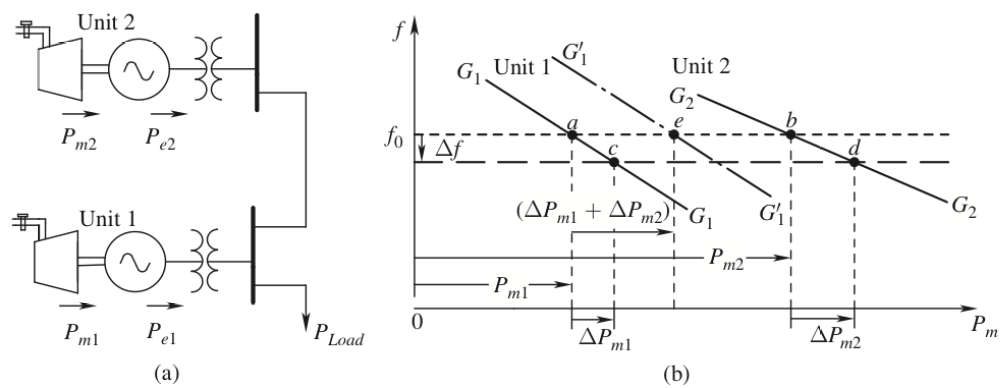
\includegraphics[width=0.7\textwidth]{images/two-gen-primary.png}
    \end{center}
    \begin{itemize}
        \item Imagine that suddenly load power increases by $\Delta P_L$: because of KL, total electric power of generators will also increase, hence they start to decelerate leading to a frequency drop. Both will react, according to the governor settings of their primary frequency control loop, to increase their mechanical power
        \item At steady state, $\Delta f$ will be such that $\Delta P_1+ \Delta P_2 = \Delta P_L$; typical time to reach steady state: 10-20s
    \end{itemize}
\end{frame}

\begin{frame}[allowframebreaks]{Share of power variation among the generators}
  
  The steady-state characteristics of the various generators can be combined into: 
  $$p_m = \sum_{i=1}^n p_{mi} = \sum_{i=1}^n \left( P_i^o - \frac{f - f_N}{f_N} \frac{P_{Ni}}{\sigma_i} \right)$$
  Expressing that load is balanced by generation, and remembering that $\Delta f = f - f_N$:
  $$\sum_{i=1}^n \left( P_i^o - \frac{\Delta f}{f_N} \frac{P_{Ni}}{\sigma_i} \right) = P_e^o (1 + D_l \Delta f)$$
  
  
  In particular, at the initial operating point, the system is assumed balanced $\sum_{i=1}^n P_i^o = P_e^o$ 
  
  A disturbance appears: an increase $\color{red}{\Delta P_e}$ of consumption, the setpoints $P_i^o$ being unchanged 
  $$\sum_{i=1}^n \left( P_i^o - \frac{\Delta f}{f_N} \frac{P_{Ni}}{\sigma_i} \right) = P_e^o (1 + D_l \Delta f) \color{red}{+ \Delta P_e}$$
  
  Which can be simplified to:
  $$-\frac{\Delta f}{f_N} \sum_{i=1}^n \frac{P_{Ni}}{\sigma_i} = P_e^o D_l \Delta f  \color{red}{+ \Delta P_e}$$
  given the relation for the initial operating point.
  
  This can be rearranged to yield:
  $$\Delta f = -\frac{\color{red}{\Delta P_e}}{\color{blue}{\beta}}$$

  with $\color{blue}{\beta} = \frac{1}{f_N} \sum_{i=1}^n \frac{P_{Ni}}{\sigma_i} +  D_l P_e^o$ 

  \begin{block}{Stiffness of system $\beta$}
    $\beta$ is called the \textit{composite frequency response characteristic} [MW/Hz], also called \textit{network power frequency characteristic} or \textit{stiffness of system}. En français: énergie régulante.
    It characterizes the accuracy of primary frequency control.
  \end{block}

  \begin{block}{Variation of power of j-th generator}
    $$\Delta P_{mj} = -\frac{\Delta f}{f_N} \frac{P_{Nj}}{ \sigma_j} = \frac{\Delta P_e P_{Nj}}{f_N \beta \sigma_j}$$
    \end{block}
            
  \begin{columns}
  \begin{column}{0.3\textwidth}  
    The steady-state frequency error allows a predictable and adjustable sharing of the power variation over the various (participating) generators 
  \end{column}
  \begin{column}{0.68\textwidth}
  \begin{itemize}
      \item all speed droops being fixed, the larger the nominal power of a generator, the larger its participation 
      \item all nominal powers being fixed, the smaller the speed droop of a generator, the larger its participation 
      \item the larger the number of generators participating in frequency control, the smaller the frequency deviation.
  \end{itemize}
  \end{column}
  \end{columns}
    
\end{frame}

% Slide 17: Primary frequency control - Primary reserve
\begin{frame}{Primary reserve}
    Only a fraction of the total number of generators participate in primary frequency control.

    To participate, the generator must have a primary reserve, i.e. it must produce less than its maximum power, and more than its minimum power
    \begin{itemize}
        \item but some units cannot (easily) vary their power: e.g. nuclear units 
        \item for generators using a renewable energy source, the amount of reserve varies and is uncertain, and they can provide only downward reserve (unless they are curtailed on purpose to provide upward reserve)
    \end{itemize}
    Primary reserve is thus a service offered by the producer on the corresponding dedicated market. If it is selected, the generator is paid.
\end{frame}

\section{Secondary frequency control (aka AGC)}


\begin{frame} {Secondary frequency control (aka AGC)}
    \begin{itemize}
        \item After (gentle and successful) settlement of primary frequency control there are however some undesirable side effects:
        \begin{itemize}
            \item Frequency has deviated from the nominal value
            \item The exchanges between areas have deviated from their scheduled values
            \item Part of the primary frequency control reserves have been depleted
        \end{itemize}
        \item AGC (or secondary frequency control) aims at cancelling these side effects:
    \end{itemize}
    \begin{itemize}
        \item Since AGC is an integral control, its steady state corresponds to zero $\Delta f$ and zero $\Delta P$ (tie-line flows are also steered back to scheduled values)
        \item Once frequency is back to normal, primary control reserves are again fully available (takes 5-15 minutes)
    \end{itemize}
\end{frame}

\begin{frame}[allowframebreaks]{Consider 2 interconnected zones}
  Each zone contains several machines, and the two zones are interconnected by a tie-line (or several tie-lines).  
  \begin{center}
        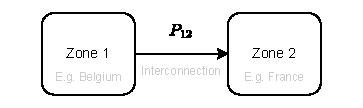
\includegraphics[width=0.7\textwidth]{images/zones.pdf} \\
    \end{center}
    
    
    With the same modelling assumptions as previously, the impact of primary frequency control is as follows:
    \begin{columns}
      \begin{column}{0.48\textwidth}
        Zone 1
        \begin{itemize}
          \item generators: $P_{m1} = \sum_{i \in 1} P_i^o - \frac{f - f_N}{f_N} \sum_{i \in 1} \frac{P_{Ni}}{\sigma_i}$ 
          \item load: $P_{e1} = P_{e1}^o + D_{l1} P_{e1}^o (f - f_N)$ 
          \item power balance: $P_{m1} = P_{e1} \color{red}{+ P_{12}}$ 
        \end{itemize}
      \end{column}
      \begin{column}{0.48\textwidth}
      Zone 2:
      \begin{itemize}
        \item generators: $P_{m2} = \sum_{i \in 2} P_i^o - \frac{f - f_N}{f_N} \sum_{i \in 2} \frac{P_{Ni}}{\sigma_i}$ 
        \item load: $P_{e2} = P_{e2}^o + D_{l2} P_{e2}^o (f - f_N)$ 
        \item power balance: $P_{m2} = P_{e2} + P_{21} = P_{e2} \color{red}{- P_{12}}$ 
      \end{itemize}
      \end{column}
    \end{columns}
    Power balance of whole system: $P_{m1} + P_{m2} = P_{e1} + P_{e2}$ 

    \begin{block}{Scenario}
    
      \begin{itemize}
        \item the whole system operates initially at frequency $f_N$ 
        \item the load power in zone 1 increases by $\Delta P_{e1}$.
      \end{itemize}
    \end{block}
  \end{frame}


\begin{frame}[allowframebreaks]{Analysis}
  Applying the relations of primary frequency control, by linearity, to the two zones, we have:
  \begin{itemize}
      \item zone 1: $-\beta_1 \Delta f = \Delta P_{e1} + \Delta P_{12}$ 
      \item zone 2: $-\beta_2 \Delta f = -\Delta P_{12}$ 
  \end{itemize}
   $\beta_1 and  \beta_2$ are composite frequency response characteristics of zones 1 and 2, respectively.
    
   Hence the frequency changes by $$\Delta f = -\frac{\Delta P_{e1}}{\beta_1 + \beta_2}$$

   The tie-line power changes by $$\Delta P_{12} = -\frac{\beta_2}{\beta_1 + \beta_2} \Delta P_{e1} < 0$$
   \begin{itemize}
      \item The power flow from zone 1 to zone 2 decreases, due to the support provided to zone 1 by the generators of zone 2 
      \item the larger $\beta_2$ with respect to $\beta_1$, the more pronounced this effect.
    \end{itemize}
\end{frame}



% Slide 20: Secondary frequency control - Objectives and Implementation
\begin{frame}{Objectives and principle of secondary frequency control}
    \begin{itemize}
        \item Eliminate the frequency error inherent to primary frequency control 
        \item Bring the power exchange between zones to the desired value (contracts) 
        \item Restore the generator primary reserves 
    \end{itemize}

In our two-zone example: 
\begin{itemize}
    \item increase the production of some generators in zone 1, where load increased 
    \item the powers of the generators in zone 2 need not be adjusted! 
\end{itemize}

\end{frame}

\begin{frame}{Implementation of secondary frequency control}
    
Acts in pre-defined control areas: 
\begin{itemize}
    \item corresponding to a country, to the zone managed by a transmission operator, etc. 
\end{itemize}

Measurements are gathered in each control area: 
\begin{itemize}
    \item frequency 
    \item sum of power flows in the tie-lines linking the area to the rest of the system 
\end{itemize}

Power \textbf{set-point} corrections $\Delta P_i^o$ are sent to dedicated generators in the area.
It is very important to note that the setpoints are corrected, not the actual power outputs of the generators.
    
\end{frame}



% Slide 21: Secondary frequency control - 
\begin{frame}{Distributed control in interconnected areas}
    %\begin{center}
    %    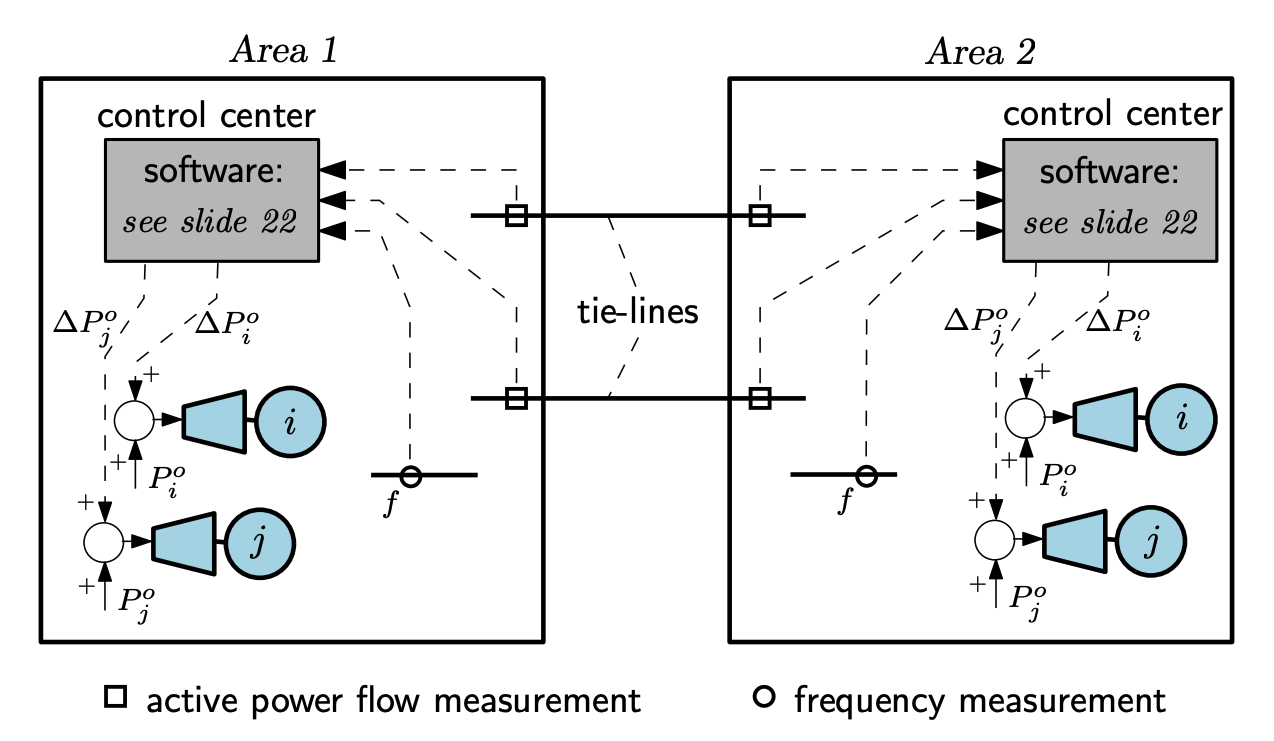
\includegraphics[width=0.7\textwidth]{images/AGC_TWO_ZONES.png} % Replace with your image file
    %\end{center}
    
    Control distributed in the various areas: 
    \begin{itemize}
      \item Measurements from one area are gathered by the control center of that area 
      \item There is no exchange of real-time measurements between areas 
    \end{itemize}
\end{frame}



% Slide 22: Secondary frequency control - ACE and PI controller
\begin{frame}{Area Control Error (ACE)}
Two-zone example, assuming zone 1 $\equiv$ area 1 and zone 2 $\equiv$ area 2. 

We define the Area Control Error (ACE) as the difference between the power exchanged on the tie-line and the desired value, plus a frequency term:  
    \begin{itemize}
        \item in area 1: $$ACE_1 = P_{12} - P_{12}^0 + {\color{blue} \lambda_1}(f - f_N) = \Delta P_{12} + {\color{blue}\lambda_1} \Delta f$$ 
        \item in area 2: $$ACE_2 = P_{21} - P_{21}^0 + {\color{blue} \lambda_2}(f - f_N) = -\Delta P_{12} + {\color{blue}\lambda_2} \Delta f$$
         
    \end{itemize}
 {\color{blue}$\lambda_1$} and {\color{blue}$\lambda_2$} are two bias factors.
\end{frame}

\begin{frame}{Generator power correction}
  It is the ouput of a Proportional-Integral controller:
    \begin{itemize}
        \item in area 1: ${\color{red} \Delta P_1^o} = -K_{p1} ACE_1 - K_{i1} \int ACE_1 dt$, \quad $K_{i1},K_{p1} > 0$ 
        \item in area 2: ${\color{red} \Delta P_2^o} = -K_{p2} ACE_2 - K_{i2} \int ACE_2 dt$, \quad $K_{i2},K_{p2} > 0$ 
    \end{itemize}
    
    The corrections is then distributed over the generators participating in secondary frequency control:
    \begin{itemize}
        \item for the i-th generator of area 1: $P_i^o + {\color{orange}\rho_i} {\color{red} \Delta P_1^o}$ with $\sum_{i} {\color{orange}\rho_i} = 1$ 
        \item for the j-th generator of area 2: $P_j^o + {\color{orange}\rho_j} {\color{red} \Delta P_2^o}$ with $\sum_{j} {\color{orange}\rho_j} = 1$ 
    \end{itemize}
\end{frame}


% Slide 23: Secondary frequency control - Steady state and bias factors
\begin{frame}{Properties}
    \begin{itemize}
        \item When the system comes back to steady state, the integral control imposes: 
        \begin{itemize}
            \item $ACE_1 = 0 \Rightarrow \Delta P_{12} + \lambda_1 \Delta f = 0$
            \item $ACE_2 = 0 \Rightarrow -\Delta P_{12} + \lambda_2 \Delta f = 0$
        \end{itemize}
        \item whose solution is: $\Delta f = 0$ and $\Delta P_{12} = 0$ 
        \item both objectives of secondary frequency control are met ! 
    \end{itemize}
  \end{frame}

\begin{frame}{Choosing the bias factors {\color{blue}$\lambda_i$}}
    \begin{itemize}
        \item They do not impact the final system state but the dynamics to reach it 
        \item It is appropriate to choose: $\lambda_1 = \beta_1$,  $\lambda_2 = \beta_2$ 
        \item Indeed, in the above example: 
        \begin{itemize}
            \item $ACE_2|_{\lambda_2=\beta_2} = -\Delta P_{12} + \beta_2 \Delta f = 0$ by definition of the primary frequency response characteristic $\beta_2$
            \item Hence $ \Delta P_2^o = 0$ all the time, since $ACE_2 = 0$ 
            \item No adjustment of the generators in zone 2,  that’s what we wanted! 
        \end{itemize}
        \item the more $\lambda_2$ differs from $\beta_2$, the more the generators in zone 2 are uselessly adjusted by the secondary frequency controller.
    \end{itemize}
\end{frame}



% Slide 24: Secondary frequency control - Gains and participation factors
\begin{frame}{Choosing the $K_i$ and $K_p$ gains of the PI controllers}
    \begin{itemize}
        \item They influence the dynamics, in particular the speed of action of secondary frequency control 
        \item secondary frequency control must not act too promptly, in order not interfere with primary frequency control (which is the “first line of defense”) 
        \item quite often, $K_p = 0$ (integral control only).
    \end{itemize}
    \subsection*{Choosing the participation factors $\rho_i$}
    \begin{itemize}
        \item $\rho_i$ coefficients: distribute the correction signal $\Delta P_1^o$ (or $\Delta P_2^o$) on the participating generators, which must have secondary reserve 
        \item for both primary and secondary frequency controls, the power variation that a participating unit commits to provide, in a given time interval, must be compatible with its maximum rate of change: 
        \begin{itemize}
            \item ' a few \% $P_N$ / min for thermal units 
            \item ' $P_N$ / min for hydro units.
        \end{itemize}
    \end{itemize}
\end{frame}




\section{Economic dispatch and optimal power flow (brief)}

% Economic dispatch problem statement (ED)
\begin{frame}
    \frametitle{Economic dispatch problem statement (ED)}
    Solve an optimization problem
    \begin{itemize}
        \item Given a total load $P_L$ to serve, and a set of candidate generators $i=1\ldots n$, with $P_i$ constrained to $\underline{P}_i \ldots \overline{P}_i$, and a cost function $C_i(P_i)$,
        \item Find optimal values $P_i$ such that $\sum_i^n C_i(P_i)$ is minimized
        \begin{itemize}
            \item while ensuring $\sum_i^n P_i = P_L$ (+ a loss term, possibly).
        \end{itemize}
        \item See 12.4.1 of ref. book for some intuition about the solution to this problem
    \end{itemize}
\end{frame}

% Optimal power flow problem statement (OPF)
\begin{frame}
    \frametitle{Optimal power flow problem statement (OPF)}
    \begin{itemize}
        \item As above, + network constraints
        \item Given
        \begin{itemize}
            \item network topology,
            \item electrical parameters of lines, cables, transformers, and shunt devices,
            \item current flow limits of lines and transformers, and voltage tolerance intervals at buses
        \end{itemize}
        \item Determine the $P_i$ such that $\sum_i^n C_i(P_i)$ is minimized
        \begin{itemize}
            \item while modeling Kirchhoff laws and enforcing the above network-wise limits
        \end{itemize}
    \end{itemize}
\end{frame}

% Primary, secondary and tertiary frequency control
\begin{frame}[allowframebreaks]{Recap}
    \begin{itemize}
        \item \textit{First}, primary control stabilizes frequency and power balance
        \begin{itemize}
            \item response within 0-30s, fully local and fully automatic
        \end{itemize}
        \item \textit{Second}, frequency and power exchanges are brought back to nominal/contractual values, and primary control reserves are restored
        \begin{itemize}
            \item response within 0.5-15 minutes, via area-control center (e.g. one country in Europe)
        \end{itemize}
        \item \textit{Third}, generation and exchange schedules are re-optimized, while restoring secondary frequency control reserves
        \begin{itemize}
            \item response within 10-60 minutes, e.g. via intraday power exchange markets
        \end{itemize}
    \end{itemize}
    \begin{center}
        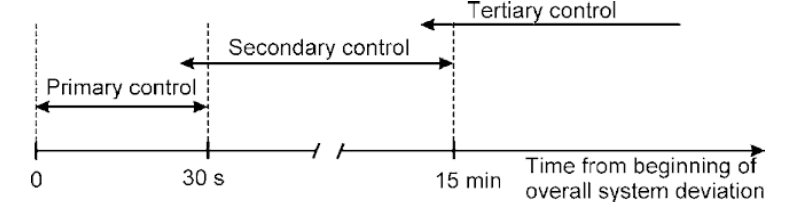
\includegraphics[width=0.65\textwidth]{images/1-2-3-freq.png}
    \end{center}
    \tiny{Fig from: \url{https://top10electrical.blogspot.com/2015/10/primary-secondary-and-tertiary.html}}
\end{frame}

\begin{frame}{Control resources}

    Which of these control resources are the main levers for freqency stability?
      \begin{itemize}
          \item Adjust synchronous generators' field current
          \item \alert{Adjust synchronous generators' mechanical power}
          \item Change transformer taps
          \item Change shunt compensation
          \item Act on topology: switch lines and transformers in/out of service
          \item \alert{Fast start-up generator units}
          \item \alert{In extremis load curtailment}
          \item \alert{Control renewable generation (e.g. PV curtailment)}
          \item \alert{Use batteries and other energy storage systems} %TODO Ask ELIA to which reserve markets batteries are participating
      \end{itemize}
\end{frame}

% Assessing the security/reliability of an electric power system
\section{Assessing the security/reliability of an electric power system (brief)}
\begin{frame}{Assessing the security/reliability of an electric power system}
    \begin{itemize}
        \item General idea of security assessment
        \item Standard \textit{N-1} static security assessment
        \item Voltage stability assessment (next lecture)
        \item Transient stability assessment (next lecture)
    \end{itemize}
\end{frame}

% General idea of security/reliability assessment
\begin{frame}[allowframebreaks]{General idea of security/reliability assessment}
    \begin{itemize}
        \item General motivation:
        \begin{itemize}
            \item Check the robustness of the system to a number of possible \textit{contingencies}
            \item NB: see examples of contingencies in subsequent slides
        \end{itemize}
        \item Generic security assessment approach:
        \begin{itemize}
            \item Given a list of contingencies and a steady-state \textit{base-case} operating point of the system
            \item Simulate the impact of each contingency if it is applied to the base case
            \item For each simulation, check whether system response is acceptable
            \item Summarize and display the results for all contingencies
            \item If \textit{too many contingencies lead to unacceptable response}, the base-case is \textit{insecure}
        \end{itemize}
        \item Remarks:
        \begin{itemize}
            \item Such analyses can be carried out periodically, based on real-time measurements
            \item They can also be applied in look-head mode, on a set of possible future system conditions
            \item Such analyses are extensively carried out by TSOs, and when the conclusion is negative, the TSO has to decide preventive/corrective counter-measures
        \end{itemize}
    \end{itemize}
\end{frame}

% Standard N-1 static security assessment
\begin{frame}[allowframebreaks]{Standard \textit{N-1} static security assessment}
    \begin{itemize}
        \item List of contingencies: all single-component outages
        \begin{itemize}
            \item e.g. all single-line outages + all single-transformer outages
            \item plus possibly all single-generator outages
        \end{itemize}
        \item Procedure:
        \begin{itemize}
            \item Run a power flow computation for the base case, and check pre-contingency limits
            \item For each outage in the contingency list, run a power flow computation to determine post-contingency voltages and currents, and check post-contingency limits
        \end{itemize}
        \item Precise limit values can depend on the context of security assessment:
        \begin{itemize}
            \item e.g. in real-time operation, line/transformer permanent thermal limits and steady state voltage magnitude tolerance intervals are checked both for pre- and post-contingency
        \end{itemize}
        \item Remarks/orders of magnitude:
        \begin{itemize}
            \item e.g. for a system like the Belgian EHV transmission system (ELIA)
            \item 1000-2000 contingencies
            \item 2000-4000 limits to check for each contingency
            \item Need to summarize in graphical form the results to be useful for a human operator
        \end{itemize}
    \end{itemize}
\end{frame}

